\documentclass[border=10pt]{standalone}
\usepackage[svgnames]{xcolor}
\usepackage{amsmath}
\usepackage{pgfplots}
\pgfplotsset{compat=newest}
\usepackage[sfdefault]{FiraSans}
\usepackage{FiraMono}
\renewcommand*\familydefault{\sfdefault}
\begin{document}
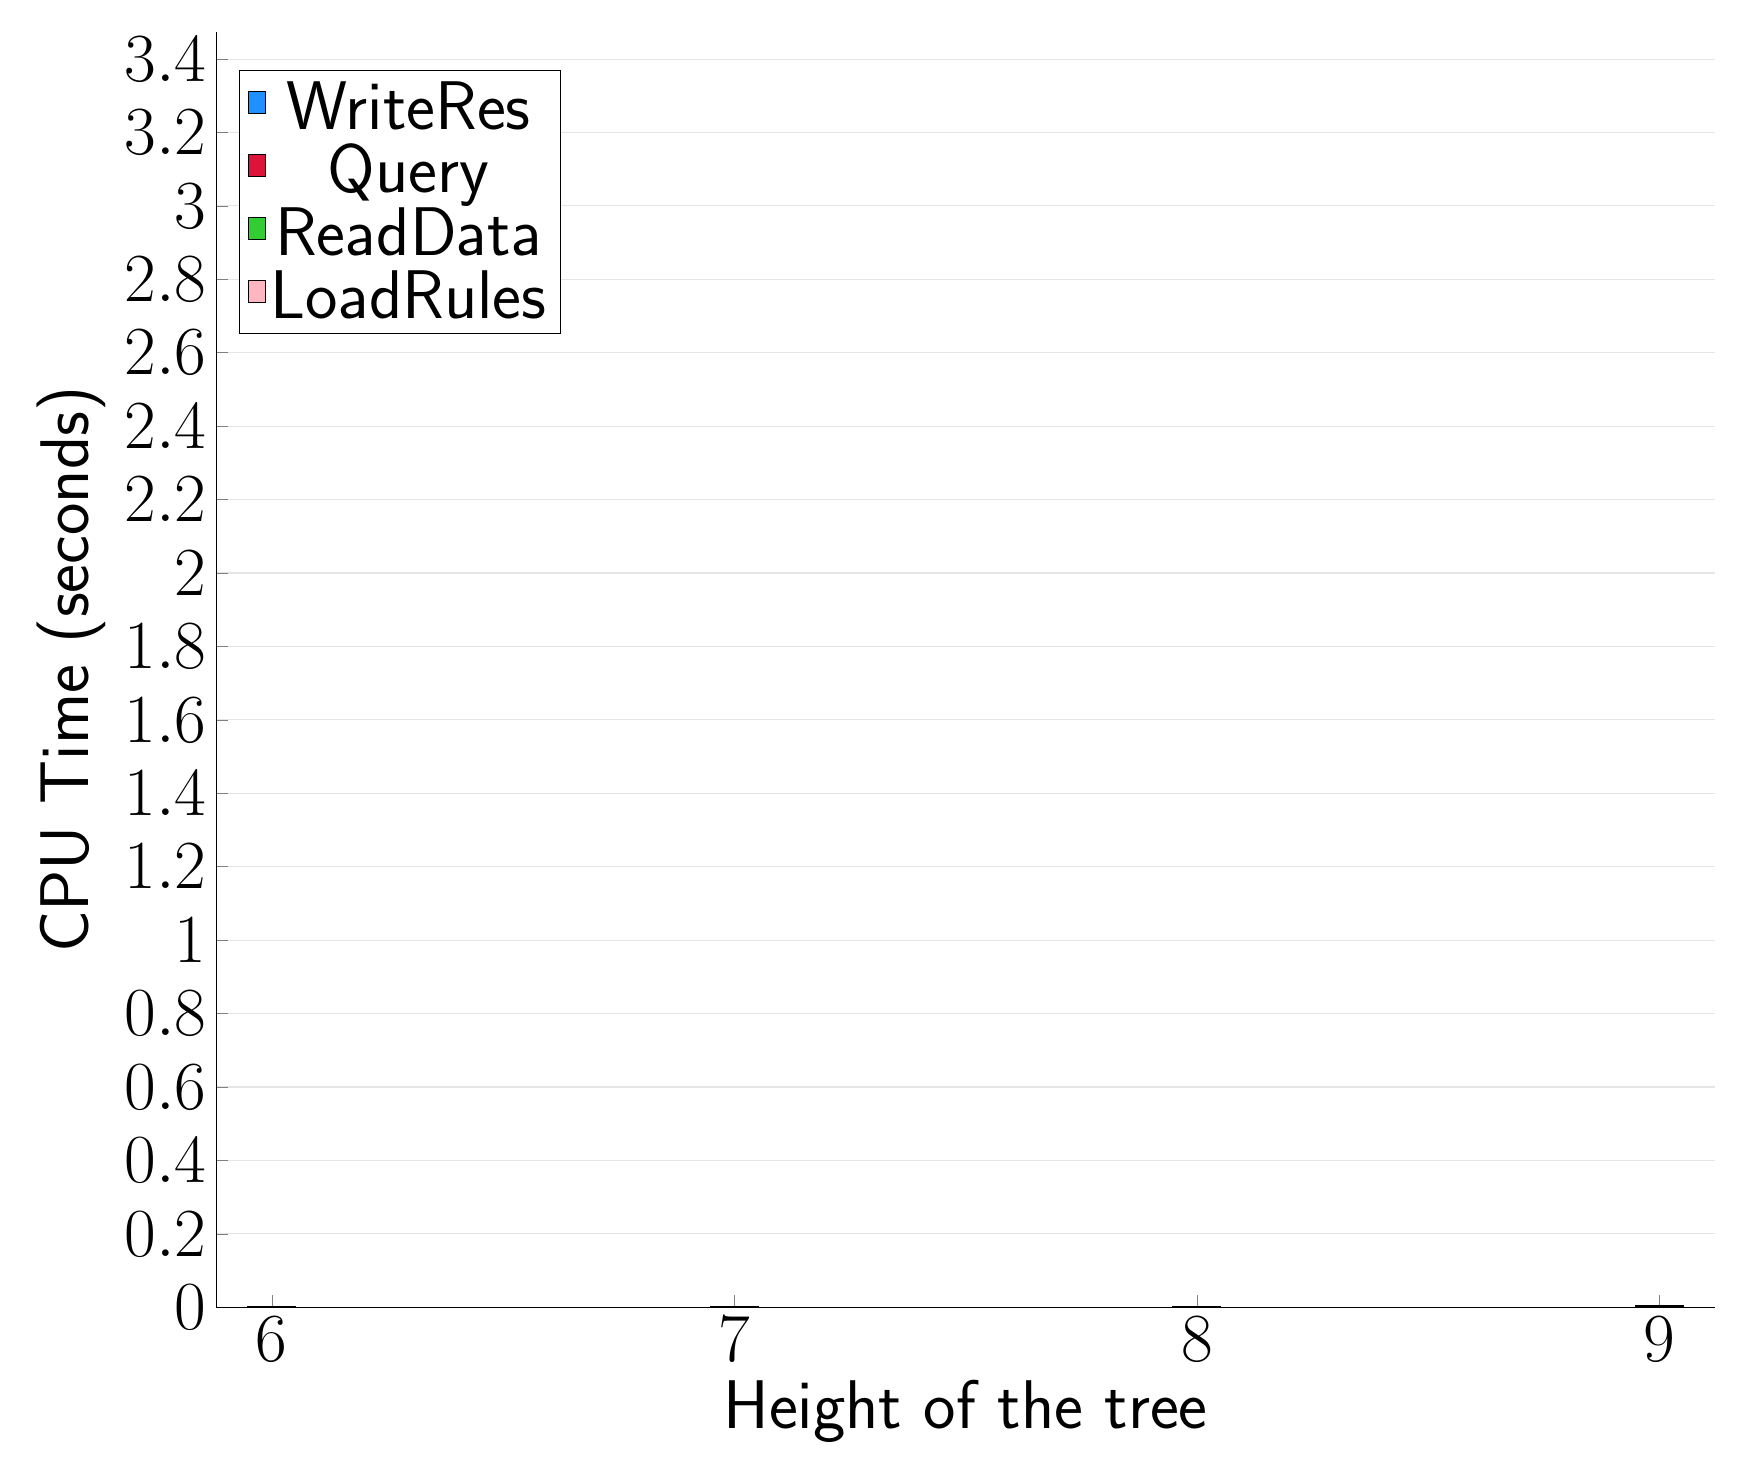
\begin{tikzpicture}
\begin{axis}[
   ybar stacked,
   width=1.7\textwidth,
   bar width=0.6cm,
   ymajorgrids, tick align=inside,
   major grid style={draw=gray!20},
   xtick=data,
   ymin=0, ymax=3.4739999999999998,
   axis x line*=bottom,
   axis y line*=left,
   enlarge x limits=0.04,
   legend style={
       at={(0.23, 0.97)},
       anchor=north east,
       legend columns=1,
       font=\Huge,
   },
   ylabel={CPU Time (seconds)},
   xlabel={Height of the tree},
   label style={font=\Huge},
   tick label style={font=\Huge},
]
\addlegendimage{fill=DodgerBlue, draw=black, line width=0.2pt}
\addlegendentry{WriteRes}
\addlegendimage{fill=Crimson, draw=black, line width=0.2pt}
\addlegendentry{Query}
\addlegendimage{fill=LimeGreen, draw=black, line width=0.2pt}
\addlegendentry{ReadData}
\addlegendimage{fill=LightPink, draw=black, line width=0.2pt}
\addlegendentry{LoadRules}
\addplot +[fill=LightPink, draw=black, line width=0.55pt] coordinates {
(6, 0.0005505999999999997)
(7, 0.0005493999999999998)
(8, 0.0005625999999999999)
(8, 0.0005575999999999998)
(8, 0.0005605999999999999)
(9, 0.0005539999999999998)
(9, 0.0005510000000000001)
(9, 0.0005509999999999996)
(9, 0.0005531999999999998)
(9, 0.0005508)
};
\addplot +[fill=LimeGreen, draw=black, line width=0.55pt] coordinates {
(6, 0.00017059999999999984)
(7, 0.0002204)
(8, 0.0003188)
(8, 0.0003188)
(8, 0.00031840000000000004)
(9, 0.0005252000000000001)
(9, 0.0005206000000000002)
(9, 0.0005180000000000007)
(9, 0.0005160000000000001)
(9, 0.0005238000000000003)
};
\addplot +[fill=Crimson, draw=black, line width=0.55pt] coordinates {
(6, 5.699999999999978e-05)
(7, 0.0001315999999999996)
(8, 0.0003355999999999996)
(8, 0.0003365999999999996)
(8, 0.0003387999999999996)
(9, 0.0008494000000000005)
(9, 0.0008407999999999998)
(9, 0.0008304)
(9, 0.0008417999999999999)
(9, 0.0008331999999999999)
};
\addplot +[fill=DodgerBlue, draw=black, line width=0.55pt] coordinates {
(6, 0.0002699999999999996)
(7, 0.0005820000000000004)
(8, 0.0013308000000000003)
(8, 0.0013108000000000002)
(8, 0.0012972000000000005)
(9, 0.0029599999999999995)
(9, 0.0029746)
(9, 0.0029761999999999996)
(9, 0.0030052000000000004)
(9, 0.0030192000000000005)
};
\end{axis}
\end{tikzpicture}

\end{document}
